% Created 2023-06-05 Mon 18:33
% Intended LaTeX compiler: pdflatex
\documentclass[11pt]{article}
\usepackage[utf8]{inputenc}
\usepackage[T1]{fontenc}
\usepackage{graphicx}
\usepackage{grffile}
\usepackage{longtable}
\usepackage{wrapfig}
\usepackage{rotating}
\usepackage[normalem]{ulem}
\usepackage{amsmath}
\usepackage{textcomp}
\usepackage{amssymb}
\usepackage{mhchem}

\author{Eric Viklund}
\date{\date}
\title{Direct Evidence of Oxide Film Formation in Nb Electropolishing Using Electrochemical Impedance Spectroscopy}


\begin{document}


\maketitle
\tableofcontents


\section{Abstract}
\label{sec:org4ffe8c0}
\textbf{Using} electrochemical impedance spectroscopy, we have devised a method of sensing the microscopic surface conditions on the surface of niobium as it is undergoing an electrochemical polishing (EP) treatment. The method uses electrochemical impedance spectroscopy (EIS) to gather information on the surface state of the electrode without disrupting the polishing reaction. The EIS data is analyzed using a so-called distribution of relaxation times (DRT) method. Using DRT, the EIS data can be deconvolved into discrete relaxation time peaks without any apriori knowledge of the electrode dynamics. By analyzing the relaxation time peaks, we are able to distinguish two distinct modes of the EP reaction. As the polishing voltage is increased, the electrode transitions from the low voltage EP mode, characterized by two relaxation time peaks, to the high voltage EP mode, characterized by three relaxation time peaks. By analyzing EPed samples, we show that samples polished in the low voltage mode have significantly higher surface roughness due to grain etching and faceting. Samples polished in the high voltage mode obtain a smooth surface finish. This shows that EIS combined with DRT analysis can be use to predict etching on EPed Nb. This method can also be performed before or during the EP, which could allow for adjustment of polishing parameters to guarantee a smooth cavity surface finish.

\section{Introduction}
\label{sec:org5ef967f}
Electropolishing (EP) is commonly used to polish Nb SRF cavities to nanometer scale surface roughness. 

EIS has been used to study the chemistry of niobium in HF electrolytes before\ref{tian_2008,ranjith2018anodic,cattarin2002nb}. However, these studies have only analyzed the spectrum using qualitative methods or traditional equivalent circuit fitting techniques. These methods have proven insufficient for explaining several important phenomenon of EP such as surface etching and spontaneous current oscillations.

In this study, we use a model-free method of analyzing the EIS spectrum called distribution of relaxation times (DRT) analysis. The advantage of this method is that the EIS spectrum can be easily characterized over a large range of polishing conditions without making any assumptions about the underlying chemical processes. 

Using this method, we are able to observe the formation of the Nb\textsubscript{2}O\textsubscript{5} layer as the polishing voltage is increased. We also show that the formation of the oxide corresponds with a reduction in surface etching by analyzing Nb samples using SEM and confocal laser microscopy.


\section{Experimental}
\label{sec:orgb71f960}

A strip of Nb foil was prepared by cleaning with alcohol. A Nb wire was used as a pseudo-electrode, since it is resistant to the EP electrolyte. The counter electrode is an aluminum rod.

The EIS measurements were performed using a BioLogic VSP-300 potentiostat.



\section{Results}
\label{sec:org4a45003}

EIS measurements reveal a complex evolution of the surface chemistry as the polishing voltage is increased through the 0.5 V to 1.0 V range. As shown in \ref{fig:nyquistplot}, at 0.5 V the system exhibits a single capacitive process. This is most likely caused by the polarization of the electrical double-layer that occurs between the Nb electrode and the electrolyte. At this low voltage, the Nb\textsubscript{2}O\textsubscript{5} has not been formed due to the low oxidation current and high concentration of HF at the surface of the electrode.

When the voltage is increased, two new features appear, an inductive loop at mid-frequencies and a second capacitive loop at low frequencies. This low frequency loop as caused by the formation of the oxide film and depletion of the HF near the electrode surface. This limits the current through the electrode at higher voltages. 

When the voltage is increased from \qty{0.78}{\volt} to \qty{0.86}{\volt} the polarization resistance changes from positive to negative as shown in \ref{fig:nyquistplot}.

\begin{figure}
  \label{fig:nyquistplot}
  
\includegraphics[]{figures/nyquist.png}
  \caption{The complex impedance of Nb. Each plot shows the different regimes of electropolishing at low voltage. A one capacitive loop, B two capacitive loops, C capacitive, inductive, and capacitive loops, D capacitive, inductive, and capacitive loop with a negative resistance.}
\end{figure}



\section{Theory}
\label{sec:org7d749e2}
An alternating voltage is applied to the niobium electrode of the form:

\begin{equation}
E=E_{0}+E_{AC}\sin(\omega*t)
\end{equation}

For small amplitudes of E\textsubscript{ac}  and assuming the system is operating at a steady-state, the electrode response to the alternating voltage can be described by a linear time-invariant system (LTI). Thus the form of the current must be:

\begin{equation}
I=I_{0}+I_{AC}\cos(\omega*t+\phi)
\end{equation}

The complex impedance of the electrode is determined by the phase difference, \(\phi\), and the ratio of the magnitudes of the AC component of the current and voltage:

\begin{flalign}
& Z=\frac{I_{AC}}{E_{AC}}*e^{j\phi}\\
& or\notag\\
& Z=Z'+jZ''
\end{flalign}

Here we use 'j' as the imaginary unit to avoid confusion with the current density frequently denoted by 'i'. Z' and Z'' are respectively the real and imaginary components of Z.



The impedance spectrum of the niobium was deconvolved using the distribution of relaxation times (DRT) method. We consider the electrode as a collection of infinitesimal discrete circuit elements. This is motivated by the fact that the electrode and its surrounding environment is a 3-dimensional object where each point on the elctrode acts independantly from every other part of the elctrode. This is in contrast with the classical view of electrochemical systems that treat the electrodes as homogeneous objects described by a finite set of discrete curcuit elements.

The fundamental elctrochemical circuit element is the RC circuit, a resistor and a capacitor in parallel, and can be described by it's time constant, \(\tau\)=RC. Taking an infinite number of RC circuits in series we obtain what is known as a Voigt circuit. The impedance of an RC circuit and of an infinite Voight circuit is given by the equations:

\begin{flalign}
  \label{eq:Zrc}
  Z_{RC}&=\frac{R}{1+j\omega\tau}\\
  Z_{Voigt} &= R + j \omega L + \int_{0}^{\infty} \frac{G(\tau) d \tau}{1 + j \omega \tau}
\end{flalign}

The function G(\(\tau\)) is the distribution of relaxation times of the measured system.

It is more convenient to rewrite the integral in a log scale, since EIS measurements are typically performed over multiple orders of magnitude.

\begin{flalign}
  \label{eq:Zdrt}
  Z=&R_{s}+j\omega L+\int_{-\infty}^{\infty}\frac{\gamma(ln\tau)dln\tau}{1+j\omega \tau}
\end{flalign}

To solve for the function \(\gamma\)(ln\(\tau\)) numerically, we discretize the problem by introducing a test function.

\begin{flalign}
  \gamma(ln\tau)&\approx\sum_{n=0}^{N}x_{n}\phi_{n}(ln\tau)\\
  Z&\approx R+j\omega L+\sum_{n=0}^{N}x_{n}\int_{-\infty}^{\infty}\frac{\phi_{n}(ln\tau)dln\tau}{1+j\omega\tau}
\end{flalign}

or in matrix form:

\begin{flalign}\label{eq:Zmatrix}
  Z=& R\mathbf{1}+\mathbf{A'x}+j(\omega L\mathbf{1}+\mathbf{A''x}) \\
  \mathbf{x}=&[x_0,x_1,\ldots,x_N]^T\\
\end{flalign}

\begin{equation}\label{eq:Aprime}
  \mathbf{A'}=\int_{-\infty}^{\infty}\frac{\phi_{n}(ln\tau)dln\tau}{1+\omega^2\tau^2}
\end{equation}

\begin{equation}\label{eq:Adoubleprime}
  \mathbf{A''}=\int_{-\infty}^{\infty}\frac{-\omega\tau\phi_{n}(ln\tau)dln\tau}{1+\omega^2\tau^2}
\end{equation}

to solve for \mathbf{x} we fit equation\textasciitilde{}\ref{eq:matrix} to the experimental impedance measurements by minimizing the square difference. The matrix \mathbf{M} is a normalization term to prevent overfitting.

\begin{flalign}
  \min_{\mathbf{x},R,L}[||Z'_{exp}-(R\mathbf{1}+\mathbf{A'x})||^2+||Z''_{exp}-(\omega L\mathbf{1}+\mathbf{A''x})||^2+|\mathbf{xMx}^{T}|]
\end{flalign}

\mathbf{M} is calculated by integrating the function G(\(\tau\)) and it's derivatives. The derivative of G is equal to the sum of the derivatives of the test functions.

\begin{flalign}
  \frac{d^{k}\gamma}{dln\tau^{k}} =& \sum_{n=0}^{N}x_{n}\frac{d^{k}\phi_{n}}{dln\tau^{k}}
\end{flalign}

We want to penalize the magnitudes of the derivatives of \(\gamma\), thus we calculate the square of the derivative and integrate.

\begin{flalign}
  (\frac{d^{k}\gamma}{dln\tau^{k}})^{2} =& \sum_{n=0}^{N}x_{n}\frac{d^{k}\phi_{n}}{dln\tau^{k}} \sum_{m=0}^{N}x_{m}\frac{d^{k}\phi_{m}}{dln\tau^{k}}\\
  \int_{0}^{\infty}(\frac{d^{k}\gamma}{dln\tau^{k}})^{2} dln\tau =& \sum_{n=0}^{N} \sum_{m=0}^{N}x_{n}x_{m} \int_{0}^{\infty} \frac{d^{k}\phi_{n}}{dln\tau^{k}} \frac{d^{k}\phi_{m}}{dln\tau^{k}} dln\tau\\
  (\mathbf{M}_{k})_{n,m} =& \int_{0}^{\infty} \frac{d^{k}\phi_{n}}{dln\tau^{k}} \frac{d^{k}\phi_{m}}{dln\tau^{k}} dln\tau\\
  \mathbf{M} =& \sum_{k=0}^{K}\lambda_{k}\mathbf{M}_{k}
\end{flalign}

The optimum values of \(\lambda\)\textsubscript{k} are not trivial to find. Higher values lead to stronger smoothing of \(\gamma\), which could lead to important details being ignored. If \(\lambda\)\textsubscript{k} is too small, the procedure will overfit to any noise in the experimental data.





\subsection{Test Function}
\label{sec:org8198a5a}

To discretize the DRT function, we use a set of Gaussian test functions evenly spaced on the log scale.

\begin{flalign}
  \phi_{n}(ln\omega) &= x_{n}e^{\frac{ln\omega-ln\omega{n}}{\mu}}
\end{flalign}

The number of test functions used in the DRT fit was set to 12 functions per decade. The minimum and maximum \omega_n for the test functions was set to a range spanning three magnitudes lower than the minimum measured frequency to the highest measured frequency. 

The width, \(\mu\), of the gaussian function is set such that the full width at half maximum (FWHM) is equal to ln\(\omega\)\textsubscript{n+1}-ln\(\omega\)\textsubscript{n-1}.




\subsection{Generalized DRT}

To completely describe the electrochemistry of niobium electropolishing two generalizations to the standard DRT procedure are necessary. The first generalization is to include inductive elements into the DRT model. Equation \ref{eq:Zrc} can be shown to be equivalent to an inductive RL circuit with the same natural frequency by negating the impedance of the RC function and adding an additional series resistor with the same resistance as the RC circuit.

\begin{flalign}
  Z_{RL} = \frac{j\frac{\omega}{\omega_{0}}R}{1+j\frac{\omega}{\omega_{0}}}\\
  Z_{RL} = R - \frac{R}{1+j\frac{\omega}{\omega_{0}}}
\end{flalign}

This means we can easily include inductive elements into the DRT model by allowing the value of G to become negative and adding a new resistor in series to account for the negative values of G. \cite{kobayashi2022extended}

\begin{flalign}
  Z=&R_{s}+R_{adj}+j\omega L+\int_{-\infty}^{\infty}\frac{\gamma(ln\tau)dln\tau}{1+j\omega \tau}\\
  R_{adj} = \int_{-\infty}^{\infty}\min{(\gamma(ln\tau),0)}dln\tau
\end{flalign}

The second generalization is the addition of positive gain elements to the model. These elements correspond to processes that release energy which leads to a negative differential resistance. These elements can be included by adding a second integral to the DRT model.

\begin{flalign}
  Z = R_{s} + R_{adj} + j\omega L + \int_{-\infty}^{\infty}\frac{\gamma_{+}(ln\tau)dln\tau}{1+j\omega \tau} + \int_{-\infty}^{\infty}\frac{\gamma_{-}(ln\tau)dln\tau}{1-j\omega \tau}
\end{flalign}

By applying the same process used to reach equation \ref{eq:Zmatrix} we arrive at the discretized form of the generalized DRT model

\begin{flalign}
  Z=& R_{s}+R_{adj}+\mathbf{A'x_{re}}+j(\omega L+\mathbf{A''x_{im}})
\end{flalign}

A' and A'' are the same integrals as before. $\gamma_{+}$ and $\gamma_{-}$ are given by the equations

\begin{flalign}
  \gamma_{+}(\ln(\omega)) = \sum_n (x_{re,n}+x_{im,n}) \phi_{n}(\ln(\omega))\\
  \gamma_{-}(\ln(\omega)) = \sum_n (x_{re,n}-x_{im,n}) \phi_{n}(\ln(\omega))
\end{flalign}


\subsection{Justification for Negative Capacitances and Resistances}

The use of negative capacitances and resistances in electrochemical systems may seem to violate the laws of physics at first glance. However, it is important to remember that the equivalent circuit is not a physical circuit that exists within the electrode. Instead, the equivalent circuit should be viewed as a mathematical tool used to extract information from the EIS spectrum. 

The meaning of negative resistances and capacitances should instead be considered from the perspective of chemical reactions. The existance of a negative capacitance somply indicates a chemical process that causes the current phase to lead the voltage phase instead of the other way around. It does not imply the existance of any inductance, although the circuit can be recreated with inductors instead of capacitors, nor the existance of a magnetic field. A negative resistance indicates a chemical process that causes the current through the electrode to decrease when the voltage is increased as is the case when there exists a blocking species such as an oxide film that lowers the overall chemical reaction rate.









\begin{figure}
  \label{fig:bodeplot}
  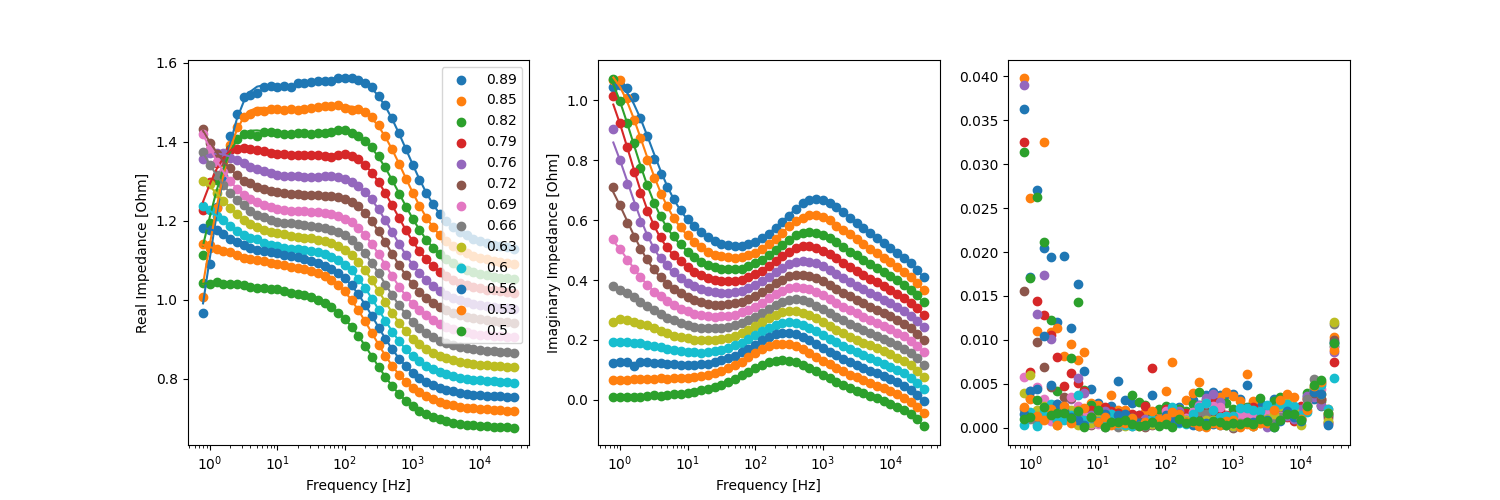
\includegraphics[]{figures/bodeplot.png}
  \caption{The complex impedance of Nb in electropolishing electrolyte measured using EIS. Each curve is offset from zero.}
\end{figure}

\begin{figure}
  \label{fig:gamma}
  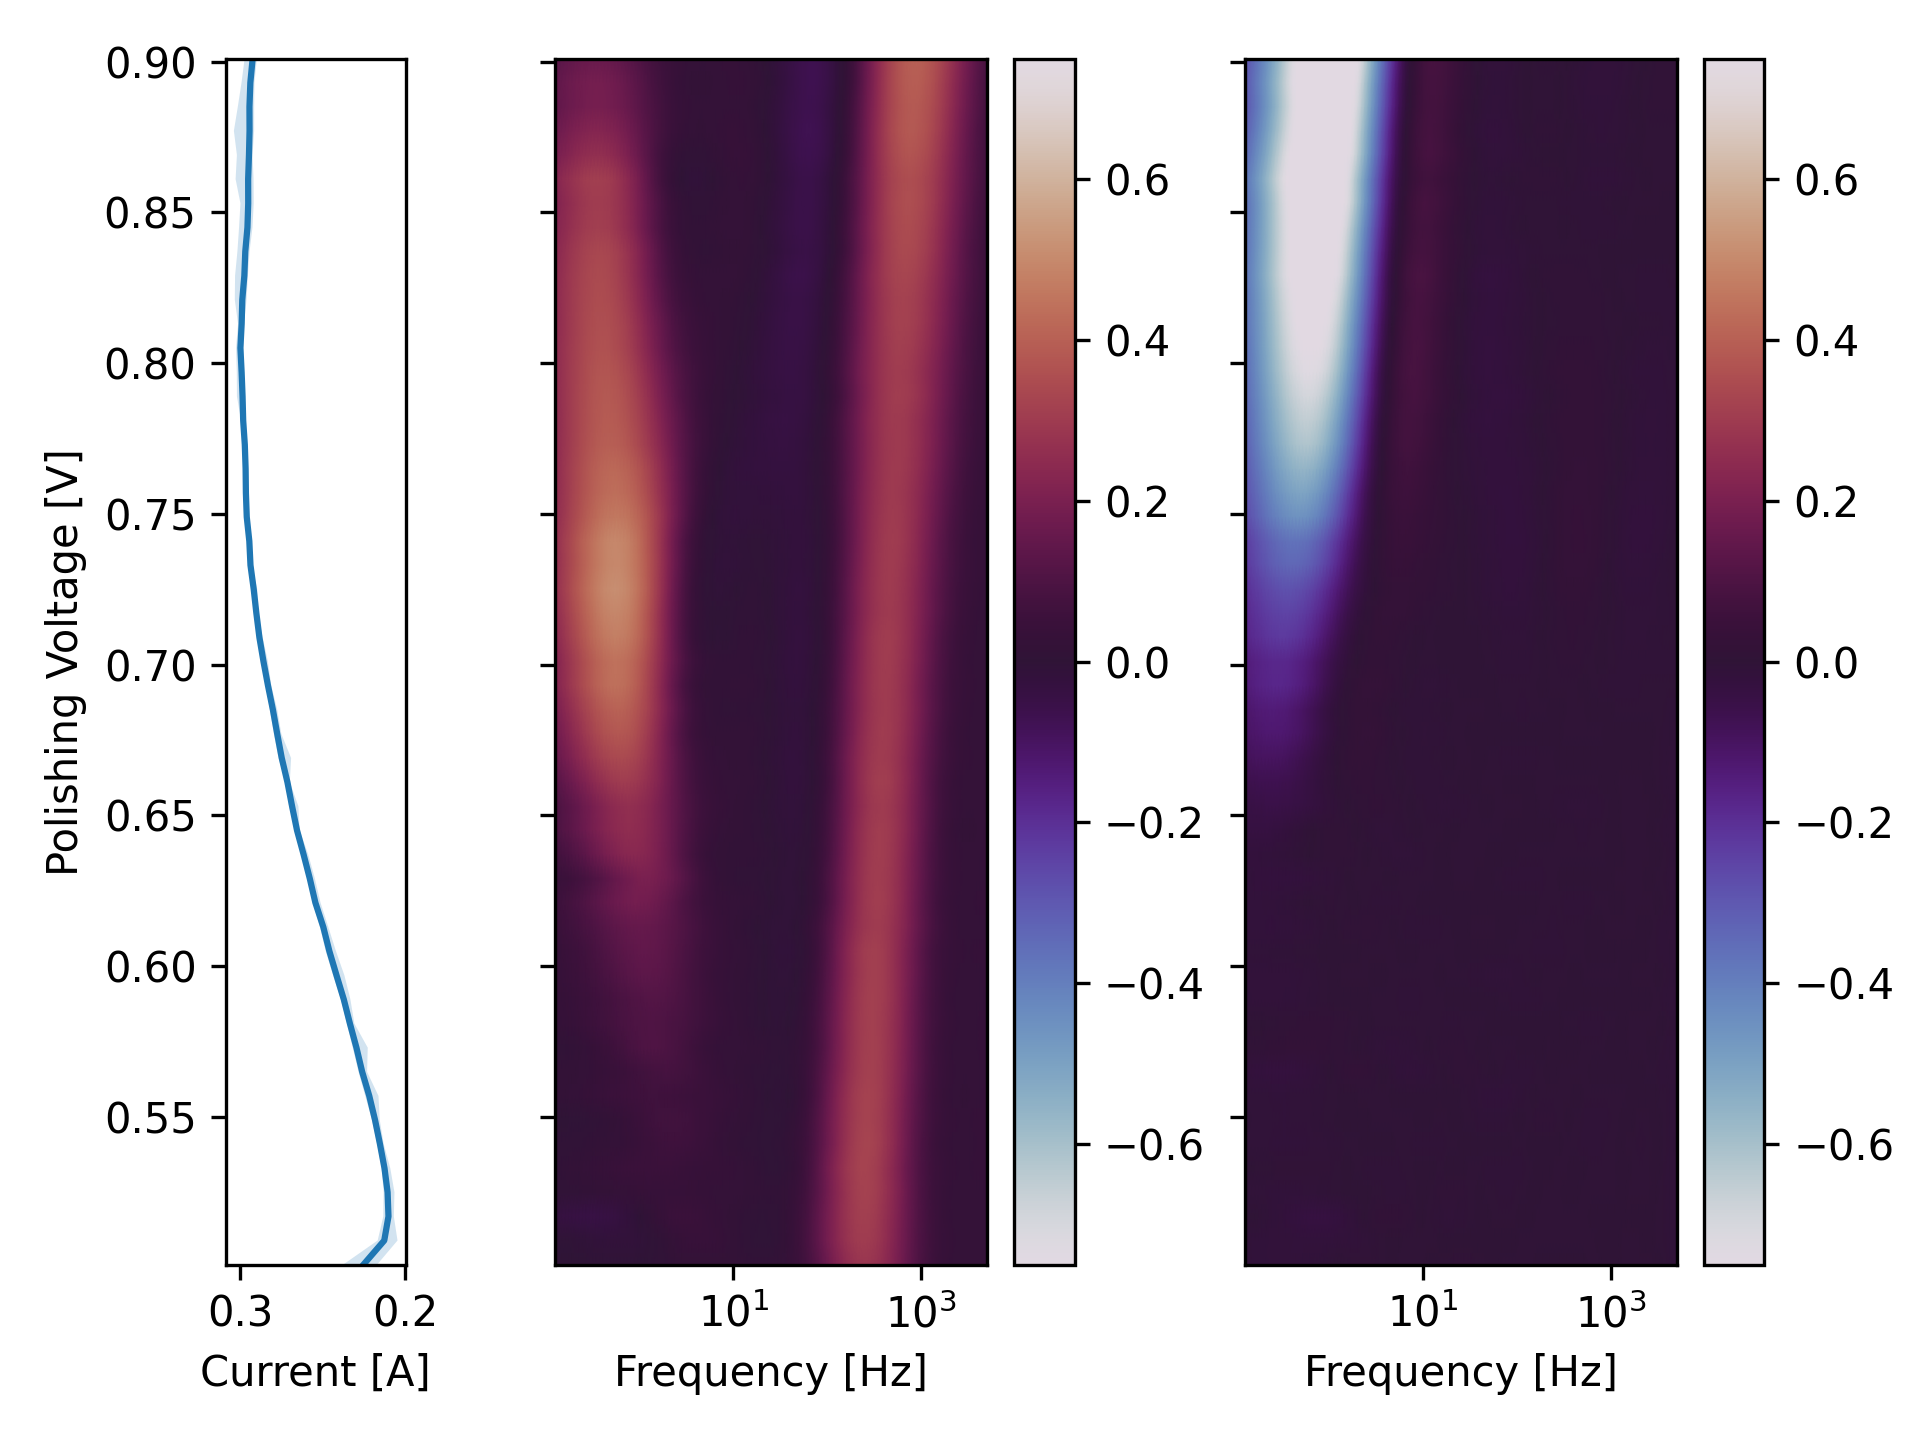
\includegraphics[]{figures/gamma.png}  
  \caption{The Distribution of relaxation times calculated from the EIS impedance data for each of the measured potentials. The current-voltage curve is shown in the graph on the left.}
\end{figure}





\subsection{Physical Interpretation of Niobium Impedance Spectrum}

The appearance of the low frequency capacitive loop is likely due to the formation of a thin compact oxide film on the niobium electrode. This occurs when the rate of oxidation exceeds the rate of oxide dissolution by the HF acid. When this happens the faradaic reaction transitions from single step to two steps. To analyze this phenomenon we propose a simplified two step oxidation reaction model where the niobium is oxidized to the V oxidation state and then chemically dissolved into the solution. In other words the average oxidation state of the oxide surface is assumed to be close to V.

\begin{flalign}
  \ce{Nb -> Nb_{V}^{5+} + 5e^-}\\
  \ce{Nb_{V}^{5+} -> Nb_{aq}}
\end{flalign}

From this reaction equation we can derive a set of differential equations that describe the dynamics of the electrode. Using the method described by Xiaojuan Wu, et al\cite{wu1998investigation,wu1999general} the surface coverage of $Nb_{V}^{5+}$ is given by the equation.

\begin{flalign}
  \beta \frac{d \theta}{dt} = g(\theta) = K_1 (1-\theta) - K_{-1} (1-\theta) - K_2 \theta\\
  i_F = 5 F \beta (1 - \theta) (K_1 - K_{-1})
\end{flalign}

\begin{flalign}
  A_1 = -5F K_2 \left(b_1 K_1 - b_{-1} K_{-1}\right)\\
  h = \frac{1}{\beta}(K_1-K_{-1}+K_2)\\
  \frac{1}{R_t} = 5F\beta K_2 \frac{b_1 K_1 - b_{-1} K_{-1}}{K_1 - K_{-1}}\\
\end{flalign}

the faradaic impedance caused by this two step reaction can be described by a resistor-inductor circuit.

\begin{flalign}
  Y_F = \frac{1}{R_t} + \frac{1}{R_1 + j \omega L_1}\\
  Y = Y_F + j \omega C_{dl}
\end{flalign}

\begin{flalign}
  A_1 = \frac{1}{L_1}\\
  h = \frac{R_1}{L_1}\\
  R_1 = \frac{h}{A_1} = -\frac{K_1 - K_{-1} + K_2}{5F \beta K_2 \left(b_1 K_1 - b_{-1} K_{-1}\right)}\\
  L_1 = \frac{1}{A_1} = -\frac{1}{5F K_2 \left(b_1 K_1 - b_{-1} K_{-1}\right)}
\end{flalign}



In the high frequency regime, the impedance is dominated by the double layer capacitance and the admittance can be reduced to the equation

\begin{flalign}
  Y = \frac{1}{R_t} + j \omega C_{dl}\\
  Z = \frac{R_t}{1 + j \frac{\omega}{\omega_{dl}}}\\
  \omega_{dl} = \frac{1}{R_t C_{dl}}
\end{flalign}

The double layer capacitance loop intersects the real axis at $Z = R_t$.

At low frequency the impedance is dominated by the faradaic impedance leading to the equation

\begin{flalign}
  Y = Y_F = \frac{1}{R_t} + \frac{1}{R_1 + j \omega L_1}\\
  Z = R_t + \frac{\frac{R_t^2}{R_1+R_t}}{1 + j \frac{\omega}{\omega_{1}}}\\
  \omega_{1} = \frac{R_1+R_t}{L_1}
\end{flalign}

The faradaic impedance loop will intersect the real axis at the value $Z = R_t + \frac{R_t^2}{R_1+R_t}$. From this equation we see that if $R_1 + R_t$ is negative, the faradaic loop will curl to the left on the nyquist diagram indicating a reduced differential resistance.

\begin{figure}
  \label{fig:ec}
  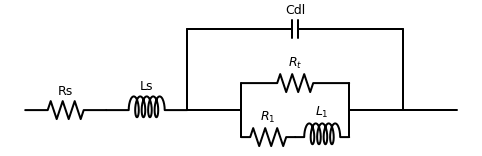
\includegraphics[]{figures/ec.png}
  \caption{}
\end{figure}


\section*{Discussion}

The negative resistance faradaic loop measured in this study could provide a reasonable explanation for the spontaneous current oscillation phenomenon encountered frequently during cavity EP. For the model analyzed in the previous section, the system is stable when the value of $h$ is positive.


\section{Conclusion}
\label{sec:org57282ed}
This study shows that EIS measurements can be used to differentiate the etching and polishing regimes in niobium EP


\section{Supplemental Information}
\label{sec:org60214d3}


\subsection{Proof of Equivalence Between Inductance and Negative Capacitance}

\subsection{Numerical Integration of \mathbf{A'} and \mathbf{A''}}
\label{sec:org84f1f26}

To calculate the matrices \mathbf{A'} and \mathbf{A''}, the integral\textasciitilde{}\ref{eq:Aprime} and\textasciitilde{} \ref{eq:Adoubleprime} must be integrated numerically. This calculation is performed using the Gaussian quadrature method.

\begin{flalign}
  \int_{a}^{b}f(x)dx \approx & \frac{b-a}{2} \sum_{i=1}^{n}w_{i}f(\frac{b-a}{2}\xi_{i}+\frac{b-a}{2})
\end{flalign}

Here \(\xi\) are the roots of the n-th Legendre polynomial and w are the weights are calculated from the derivative of the n-th Legendre polynomial using the equation

\begin{flalign}
  w_{i} =& -\frac{2}{(1-\xi_{i}^{2})(P'_{n}(\xi_{i}))}
\end{flalign}




\end{document}